\subsection{Chức năng phản hồi bình luận}
\subsubsection{Sơ đồ use-case}
\begin{figure}[H]
    \centering
    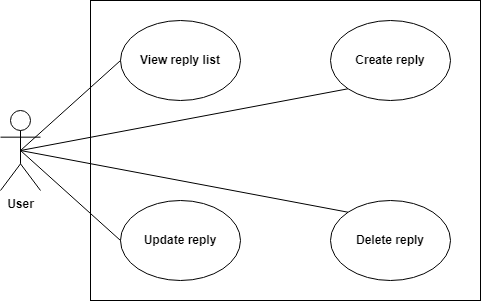
\includegraphics[width=0.7\textwidth]{Images/UseCase/Reply.png}
    \caption{Sơ đồ use-case cho các chức năng phản hồi bình luận}
\end{figure}
\subsubsection{Đặc tả use-case cho chức năng tạo phản hồi mới bình luận}
\begin{center}
    \arrayrulecolor{cyan!75!black}
    \arrayrulewidth=2pt
    \begin{longtable}{
        |>{\raggedright\arraybackslash}p{3cm}
        |>{\raggedright\arraybackslash}p{13cm}
        |}
        \hline
        \rowcolor{cyan!75!black} \textcolor{white}{\textbf{Use-case name}} & \textcolor{white}{\textbf{TẠO PHẢN HỒI MỚI CHO BÌNH LUẬN}}
        \\\hline
        \rowcolor{cyan!10!white} \textit{Actor} & Người dùng
        \\\hdashline
        \rowcolor{cyan!10!white} \textit{Description} & Tính năng cho phép người dùng tạo mới một phản hồi đối với một bình luận nhất định.
        \\\hdashline
        \rowcolor{cyan!10!white} \textit{Preconditions} & Người dùng đã đăng nhập thành công vào ứng dụng. Tồn tại ít nhất một bình luận đối với một bài đăng tải nhà thuê nhất định.
        \\\hdashline
        \rowcolor{cyan!10!white} \textit{Postconditions} & Phản hồi bình luận cho một bình luận nhất định được ghi nhận thành công.
        \\\hdashline
        \rowcolor{cyan!10!white} \textit{Trigger} & Người dùng chọn vào mục \textbf{Thêm phản hồi bình luận} ở dưới một bình luận nhất định.
        \\\hdashline
        \rowcolor{cyan!10!white} \textit{Main flow} &
        1. Ứng dụng hiển thị các trường thông tin yêu cầu người dùng cung cấp khi tạo mới một phản hồi bình luận. \newline
        2. Người dùng nhập vào nội dung cho phần phản hồi bình luận. \newline
        3. Người dùng nhấn vào mục \textbf{Tạo phản hồi bình luận}. \newline
        4. Ứng dụng kiểm tra và xử lý các trường thông tin do người dùng cung cấp. \newline
        5. Ứng dụng thông báo đăng tải phản hồi bình luận thành công.
        \\\hdashline
        \rowcolor{cyan!10!white} \textit{Alternative flow} & 
        \textbf{Nếu người dùng hủy đăng tải phản hồi bình luận, ứng dụng sẽ quay trở lại giao diện chính} \newline
        2a.1. Người dùng hủy quá trình đăng tải phản hồi bình luận. \newline
        2a.2. Ứng dụng quay trở lại giao diện chính.
        \\\hdashline
        \rowcolor{cyan!10!white} \textit{Exception flow} & 
        \textbf{Nếu thông tin phản hồi bình luận không được cung cấp đầy đủ, ứng dụng sẽ hiển thị lỗi và yêu cầu người dùng cung cấp lại thông tin} \newline
        4a.1. Ứng dụng thông báo thông tin của phản hồi bình luận chưa đầy đủ. \newline
        4a.2. Người dùng bổ sung thông tin cho phản hồi bình luận. \newline
        4a.3. Ứng dụng kiểm tra thông tin đã nhập. \newline
        4a.4. Nếu thông tin hợp lệ, ứng dụng sẽ thông báo đăng tải phản hồi bình luận thành công, ngược lại sẽ quay lại bước 2. \newline
        \textbf{Nếu thông tin đăng tải phản hồi bình luận không hợp lệ, ứng dụng sẽ hiển thị lỗi và yêu cầu người dùng cung cấp lại thông tin} \newline
        4a.1. Ứng dụng thông báo thông tin của phản hồi bình luận không hợp lệ. \newline
        4a.2. Người dùng chỉnh sửa thông tin phản hồi bình luận. \newline
        4a.3. Ứng dụng kiểm tra thông tin đã nhập. \newline
        4a.4. Nếu thông tin hợp lệ, ứng dụng sẽ thông báo đăng tải phản hồi bình luận thành công, ngược lại sẽ quay lại bước 2. \newline
        \textbf{Nếu ứng dụng gặp lỗi trong quá trình đăng tải phản hồi bình luận, ứng dụng thông báo lỗi và yêu cầu người dùng thử lại sau} \newline
        4c.1. Ứng dụng hiện lỗi khi thực hiện đăng tải phản hồi bình luận. \newline
        4c.2. Ứng dụng thông báo yêu cầu người dùng thử lại sau.
        \\\hline
        \caption{Đặc tả use-case cho chức năng tạo phản hồi bình luận mới cho bình luận}
    \end{longtable}
\end{center}
\subsubsection{Đặc tả use-case cho chức năng chỉnh sửa phản hồi bình luận}
\begin{center}
    \arrayrulecolor{cyan!75!black}
    \arrayrulewidth=2pt
    \begin{longtable}{
        |>{\raggedright\arraybackslash}p{3cm}
        |>{\raggedright\arraybackslash}p{13cm}
        |}
        \hline
        \rowcolor{cyan!75!black} \textcolor{white}{\textbf{Use-case name}} & \textcolor{white}{\textbf{CHỈNH SỬA PHẢN HỒI BÌNH LUẬN}}
        \\\hline
        \rowcolor{cyan!10!white} \textit{Actor} & Người dùng
        \\\hdashline
        \rowcolor{cyan!10!white} \textit{Description} & Tính năng cho phép người dùng chỉnh sửa một phản hồi bình luận có sẵn của người dùng đối với một bình luận nhất định.
        \\\hdashline
        \rowcolor{cyan!10!white} \textit{Preconditions} & Người dùng đã đăng nhập thành công vào ứng dụng. Người dùng có ít nhất một phản hồi bình luận đối với một bình luận nhất định.
        \\\hdashline
        \rowcolor{cyan!10!white} \textit{Postconditions} & Phản hồi bình luận được cập nhật thành công.
        \\\hdashline
        \rowcolor{cyan!10!white} \textit{Trigger} & Người dùng chọn vào mục \textbf{Chỉnh sửa phản hồi bình luận} ở phần phản hồi bình luận của người dùng.
        \\\hdashline
        \rowcolor{cyan!10!white} \textit{Main flow} &
        1. Ứng dụng hiển thị thông tin hiện tại của phản hồi bình luận của người dùng. \newline
        2. Người dùng nhập vào nội dung muốn thay đổi cho phần phản hồi. \newline
        3. Người dùng nhấn vào mục \textbf{Cập nhật phản hồi bình luận}. \newline
        4. Ứng dụng kiểm tra và xử lý các trường thông tin do người dùng cung cấp. \newline
        5. Ứng dụng thông báo cập nhật phản hồi bình luận thành công.
        \\\hdashline
        \rowcolor{cyan!10!white} \textit{Alternative flow} & 
        \textbf{Nếu người dùng hủy cập nhật phản hồi bình luận, ứng dụng sẽ quay trở lại giao diện chính} \newline
        2a.1. Người dùng hủy quá trình cập nhật phản hồi bình luận. \newline
        2a.2. Ứng dụng quay trở lại giao diện chính.
        \\\hdashline
        \rowcolor{cyan!10!white} \textit{Exception flow} & 
        \textbf{Nếu thông tin phản hồi bình luận bị bỏ trống, ứng dụng sẽ hiển thị lỗi và yêu cầu người dùng cung cấp lại thông tin} \newline
        4a.1. Ứng dụng thông báo thông tin của phản hồi bình luận bị bỏ trống. \newline
        4a.2. Người dùng bổ sung thông tin cho phản hồi bình luận. \newline
        4a.3. Ứng dụng kiểm tra thông tin đã nhập. \newline
        4a.4. Nếu thông tin hợp lệ, ứng dụng sẽ thông báo cập nhật phản hồi bình luận thành công, ngược lại sẽ quay lại bước 2. \newline
        \textbf{Nếu thông tin cập nhật cho phản hồi bình luận không hợp lệ, ứng dụng sẽ hiển thị lỗi và yêu cầu người dùng cung cấp lại thông tin} \newline
        4a.1. Ứng dụng thông báo thông tin cập nhật phản hồi bình luận không hợp lệ. \newline
        4a.2. Người dùng chỉnh sửa thông tin phản hồi bình luận. \newline
        4a.3. Ứng dụng kiểm tra thông tin đã nhập. \newline
        4a.4. Nếu thông tin hợp lệ, ứng dụng sẽ thông báo cập nhật phản hồi bình luận thành công, ngược lại sẽ quay lại bước 2. \newline
        \textbf{Nếu ứng dụng gặp lỗi trong quá trình cập nhật phản hồi bình luận, ứng dụng thông báo lỗi và yêu cầu người dùng thử lại sau} \newline
        4c.1. Ứng dụng hiện lỗi khi thực hiện cập nhật phản hồi bình luận. \newline
        4c.2. Ứng dụng thông báo yêu cầu người dùng thử lại sau.
        \\\hline
        \caption{Đặc tả use-case cho chức năng chỉnh sửa phản hồi bình luận}
    \end{longtable}
\end{center}
\subsubsection{Đặc tả use-case cho chức năng xóa phản hồi bình luận}
\begin{center}
    \arrayrulecolor{cyan!75!black}
    \arrayrulewidth=2pt
    \begin{longtable}{
        |>{\raggedright\arraybackslash}p{3cm}
        |>{\raggedright\arraybackslash}p{13cm}
        |}
        \hline
        \rowcolor{cyan!75!black} \textcolor{white}{\textbf{Use-case name}} & \textcolor{white}{\textbf{XÓA PHẢN HỒI BÌNH LUẬN}}
        \\\hline
        \rowcolor{cyan!10!white} \textit{Actor} & Người dùng
        \\\hdashline
        \rowcolor{cyan!10!white} \textit{Description} & Tính năng cho phép người dùng xóa một phản hồi bình luận của một bình luận nhất định.
        \\\hdashline
        \rowcolor{cyan!10!white} \textit{Preconditions} & Người dùng đã đăng nhập thành công vào ứng dụng. Người dùng có ít nhất một phản hồi bình luận đối với một bình luận nhất định.
        \\\hdashline
        \rowcolor{cyan!10!white} \textit{Postconditions} & Phản hồi bình luận của người dùng được xóa thành công.
        \\\hdashline
        \rowcolor{cyan!10!white} \textit{Trigger} & Người dùng chọn vào một phản hồi bình luận nhất định do người dùng đó đăng tải và chọn mục \textbf{Xóa phản hồi bình luận}.
        \\\hdashline
        \rowcolor{cyan!10!white} \textit{Main flow} &
        1. Ứng dụng hiển thị phản hồi bình luận hiện tại của người dùng. \newline
        3. Người dùng nhấn vào mục \textbf{Xóa phản hồi bình luận}. \newline
        4. Ứng dụng yêu cầu người dùng xác nhận việc xóa phản hồi bình luận. \newline
        5. Người dùng xác nhận việc xóa phản hồi bình luận. \newline
        6. Ứng dụng thông báo xóa phản hồi bình luận thành công.
        \\\hdashline
        \rowcolor{cyan!10!white} \textit{Alternative flow} & 
        \textbf{Nếu người dùng hủy xóa phản hồi bình luận, ứng dụng sẽ quay trở lại giao diện chính} \newline
        2a.1. Người dùng hủy quá trình xóa phản hồi bình luận. \newline
        2a.2. Ứng dụng quay trở lại giao diện chính.
        \\\hdashline
        \rowcolor{cyan!10!white} \textit{Exception flow} & 
        \textbf{Nếu ứng dụng gặp lỗi trong quá trình xóa phản hồi bình luận, ứng dụng thông báo lỗi và yêu cầu người dùng thử lại sau} \newline
        4c.1. Ứng dụng hiện lỗi khi thực hiện xóa phản hồi bình luận. \newline
        4c.2. Ứng dụng thông báo yêu cầu người dùng thử lại sau.
        \\\hline
        \caption{Đặc tả use-case cho chức năng xóa phản hồi bình luận}
    \end{longtable}
\end{center}